\documentclass[12pt, a4paper]{article}

% --- Packages ---
\usepackage[utf8]{inputenc}
\usepackage{geometry}
\geometry{a4paper, margin=1in}
\usepackage{setspace} 
\onehalfspacing 

\usepackage{graphicx} 
\usepackage{booktabs} 
\usepackage{enumitem} 
\usepackage{hyperref} 
\usepackage{amsmath} 
\usepackage{float} 
\usepackage{adjustbox}

\hypersetup{
	colorlinks=true,
	linkcolor=black,
	filecolor=magenta,      
	urlcolor=blue,
	citecolor=black,
}

\usepackage{parskip} 
\setlength{\parskip}{0.5em} 

\usepackage{listings}
\usepackage{xcolor}

\definecolor{codegreen}{rgb}{0,0.6,0}
\definecolor{codegray}{rgb}{0.5,0.5,0.5}
\definecolor{codepurple}{rgb}{0.58,0,0.82}
\definecolor{backcolour}{rgb}{0.95,0.95,0.92}

\lstdefinestyle{Rstyle}{
	backgroundcolor=\color{backcolour},   
	commentstyle=\color{codegreen},
	keywordstyle=\color{blue},
	numberstyle=\tiny\color{codegray},
	stringstyle=\color{codepurple},
	basicstyle=\ttfamily\footnotesize,
	breakatwhitespace=false,         
	breaklines=true,                 
	captionpos=b,                    
	keepspaces=true,                 
	numbers=left,                    
	numbersep=5pt,                  
	showspaces=false,                
	showstringspaces=false,
	showtabs=false,                  
	tabsize=2
}
\lstset{style=Rstyle}

\title{\textbf{Replication Project}}
\author{Hanyu Li (ID: 25346841)}
\date{\today}

\begin{document}
	
	\maketitle
	\thispagestyle{empty} 
	
	\newpage
	\tableofcontents
	\newpage
	
	\section{Original Research}
	
	\subsection{Research Background and Questions}
	I replicated the study by Carsten Schwemmer and Magdalena Riedl, published in 2025 in PLOS One, From hashtags to ballots: Conceptualizing political influencers and evaluating their impact on election outcomes.
	
	Theoretically, some studies have shown that political participation on social media can have a significant impact on political outcomes, particularly regarding voter turnout and political efficacy (Liebhart and Bernhardt, 2017). However, this participation often suffers from self-selection, where citizens who are already politically active dominate the online discourse (Kroh and Neiss, 2012). It remains unclear whether political messaging and campaigning can effectively reach ordinary users who lack political motivation and successfully mobilize their political participation.
	
	In reality, a new class of grassroots influencers has emerged on the internet. These individuals are different from institutional elites, such as politicians or journalists, because they do not have an official professional background in the political system. These influencers usually start by sharing non-political content about their daily lives to build a large fan base. However, during election periods, they reveal a dual nature of commercial monetization and political messaging. They continue to run product advertisements while simultaneously using their reach to shape political opinions.
	
	This paper thereby defines political influencers as ordinary internet users who accumulate a large following by narrating their personal lifestyles. They monetize their profiles by integrating advertorials into their posts but also include political topics or events in their regular content. The objective is to analyze how these influencers manage the balance between their political and commercial posts and to evaluate whether they can successfully reach voters who normally have low interest in politics.
	
	Based on the background, this study addresses the following primary research questions(I chose the most relevant ones to model replication):
	
	Research questions regarding content strategy:
	\begin{itemize}[itemsep=0.5em]
		\item \textbf{RQ2: To what extent do political influencers support or disapprove political actors or events?}
		\item \textbf{RQ3: How much advertisement is included in the posts of political influencers?}
	\end{itemize}
	
	Research questions regarding audience of political influencers:
	\begin{itemize}[itemsep=0.5em]
		\item \textbf{RQ4: Which voters are following the content of influencers?}
	\end{itemize}
	
	\subsection{Methodology}
	This study employs a mixed-methods approach utilizing two primary datasets:\\
	\textbf{1. Instagram Post Descriptive Analysis} \\
	\textbf{Data source:} The researchers constructed the Instagram dataset by scraping 3,164 image and video posts via the Instagram API between June and September 2021. They selected 98 political influencers based in Germany according to their account content, biographies, hashtags, and follower counts. To categorize the data, the authors recruited 357 coders to cross-code the posts. After data cleaning, they obtained a final dataset of 2,915 posts, which included account information, content types, and traffic metrics.
	
	\textbf{Analytical approach:} The authors used descriptive statistics to calculate the proportion of different content types and visualized how these content themes evolved weekly during the 2021 German Federal Election.
	
	\vspace{1em}
	
	\textbf{2. Logistic Regression Analysis} \\
	\textbf{Data source:} The authors utilized data from an online follow-up survey conducted for the 2021 German Federal Election. The survey included 2,891 respondents and covered demographic variables, social media usage patterns, awareness of political influencers, and political participation behaviors.
	
	\textbf{Analytical approach:} The researchers employed two binary logistic regression models to analyze the effects of social media motivations, political interest, and control variables (age, education, and the number of social media platforms used) on respondents' likelihood of being aware of and following political influencers.
	
	\textbf{Model Equations:} 
	\begin{align*}
		\begin{aligned}
			\text{Model 1 (Awareness):} \quad \ln\left(\frac{P_{\text{aware}}}{1-P_{\text{aware}}}\right) &= \alpha + \beta_1 \text{PolInt} + \beta_2 \text{MotivPublic} + \beta_3 \text{MotivBrand} \\
			&\quad + \beta_4 \text{MotivEntertain} + \beta_5 \text{Controls} \\[1.5em]
			\text{Model 2 (Following):} \quad \ln\left(\frac{P_{\text{follow}}}{1-P_{\text{follow}}}\right) &= \gamma_0 + \gamma_1 \text{PolInt} + \gamma_2 \text{MotivPublic} + \gamma_3 \text{MotivBrand} \\
			&\quad + \gamma_4 \text{MotivEntertain} + \gamma_5 \text{Controls}
		\end{aligned}
	\end{align*}
	
	\textbf{Variable Coding:}
	
	\begin{itemize}[itemsep=0.3em]
		
		\item \textbf{Dependent Variables:}
		
		\begin{itemize}
			
			\item \textbf{Awareness (\texttt{influ\_aware}):} Binary variable (0 = unaware, 1 = aware), with ``unaware'' as the baseline.
			
			\item \textbf{Following (\texttt{influ\_follow}):} Binary variable (0 = not following, 1 = following), with ``not following'' as the baseline.
			
		\end{itemize}
		
		\item \textbf{Independent Variables:}
		
		\begin{itemize}
			
			\item \textbf{Political Interest:} Likert scale (1 = low, 5 = high).
			
			\item \textbf{Social Media Motivations:} Three separate Likert scale variables (1-5) measuring motivations for following public figures, following brands, and seeking entertainment.
			
		\end{itemize}
		
		\item \textbf{Control Variables:}
		
		\begin{itemize}
			
			\item \textbf{Age:} Continuous variable in years.
			
			\item \textbf{Education:} Categorical variable (1 = low, 2 = mid, 3 = high), with ``low'' as the baseline.
			
			\item \textbf{SM Platforms Used (\texttt{sm\_cnt}):} Continuous variable measuring the count of active social media platforms.
			
		\end{itemize}
		
	\end{itemize}
	
	\textbf{Hypotheses (Unified):} \\
	\textbf{Model 1 (Awareness):}
	\begin{itemize}[itemsep=0em]
		\item $H_0: \beta_1 = \beta_2 = \dots = \beta_9 = 0$
		\item $H_a:$ at least one coefficient $\neq 0$
	\end{itemize}
	
	\textbf{Model 2 (Following):}
	\begin{itemize}[itemsep=0em]
		\item $H_0: \gamma_1 = \gamma_2 = \dots = \gamma_9 = 0$
		\item $H_a:$ at least one coefficient $\neq 0$
	\end{itemize}
	
	\section{Replication}
	
	\subsection{Instagram Post Descriptive Analysis}
	\lstinputlisting[language=R, firstline=47, lastline=138]{replication.R}
	
	\begin{figure}[H]
		\centering
		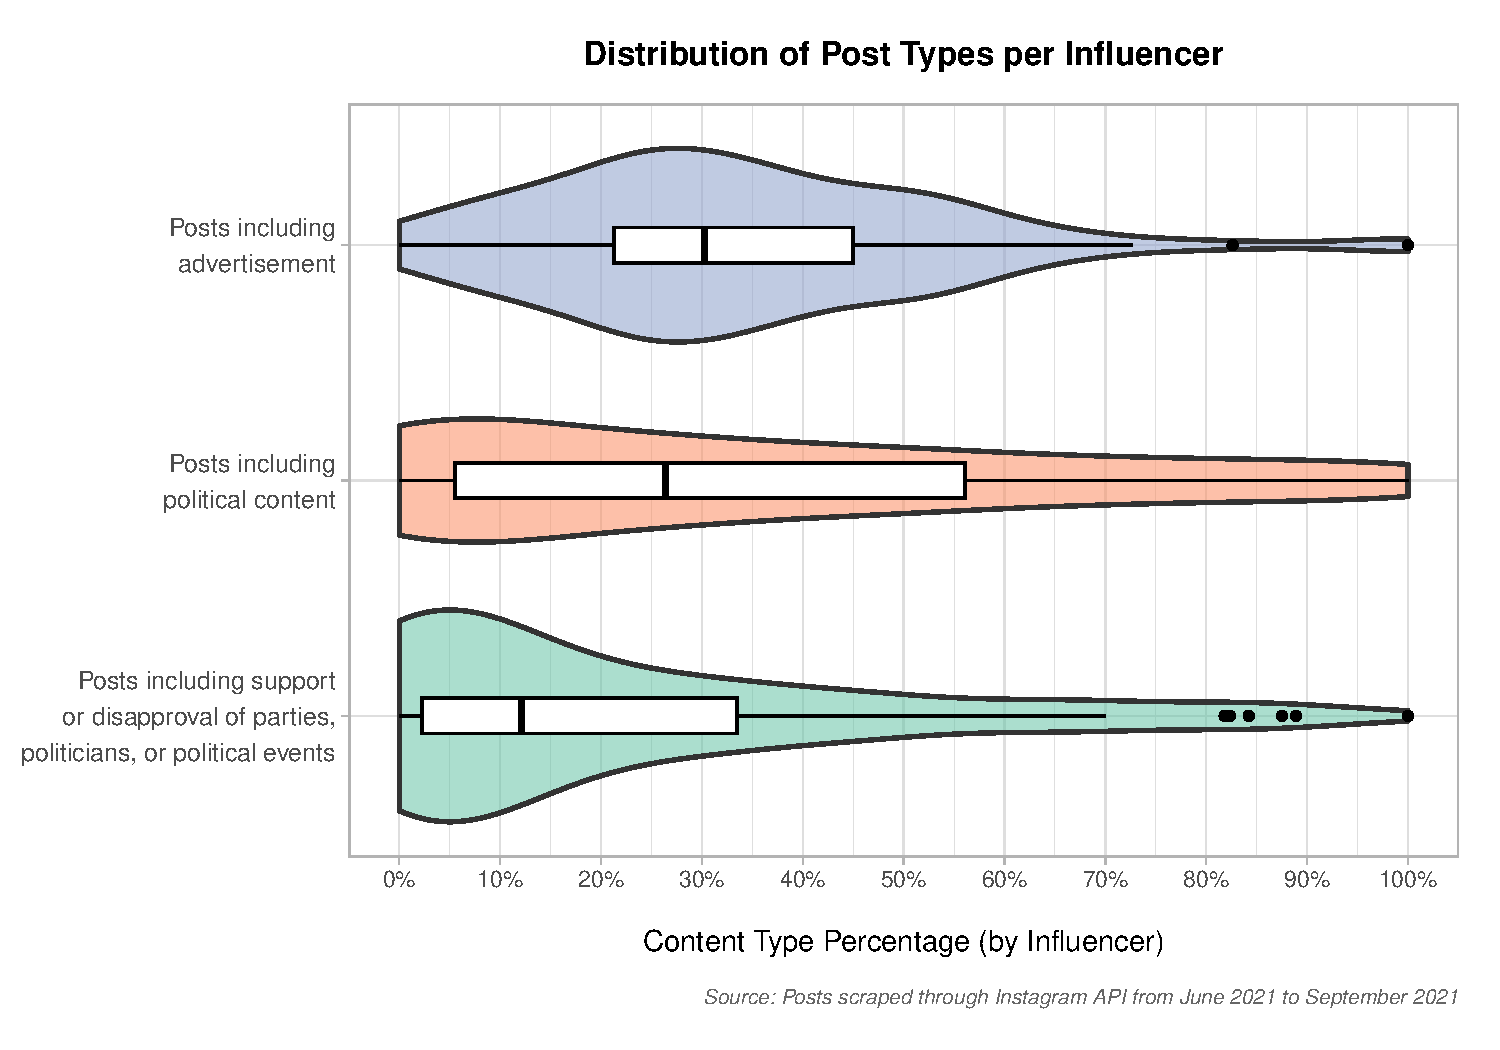
\includegraphics[width=0.85\textwidth]{fig2_rep.pdf}
		\caption{Distribution of post types across influencers.}
		\label{fig:2}
	\end{figure}
	
	Figure \ref{fig:2} utilizes violin plots to illustrate the distribution of post types across influencers, with the width of the violins representing the density of influencers at each percentage level. For this replication, I explicitly annotated the data source to enhance transparency. The authors conclude from this distribution that while influencers frequently integrate commercial advertisements into their feeds, explicit support or disapproval of specific political actors remains notably scarce, thereby illustrating the dual nature of commercial monetization and political messaging among political influencers.
	
	\begin{figure}[H]
		\centering
		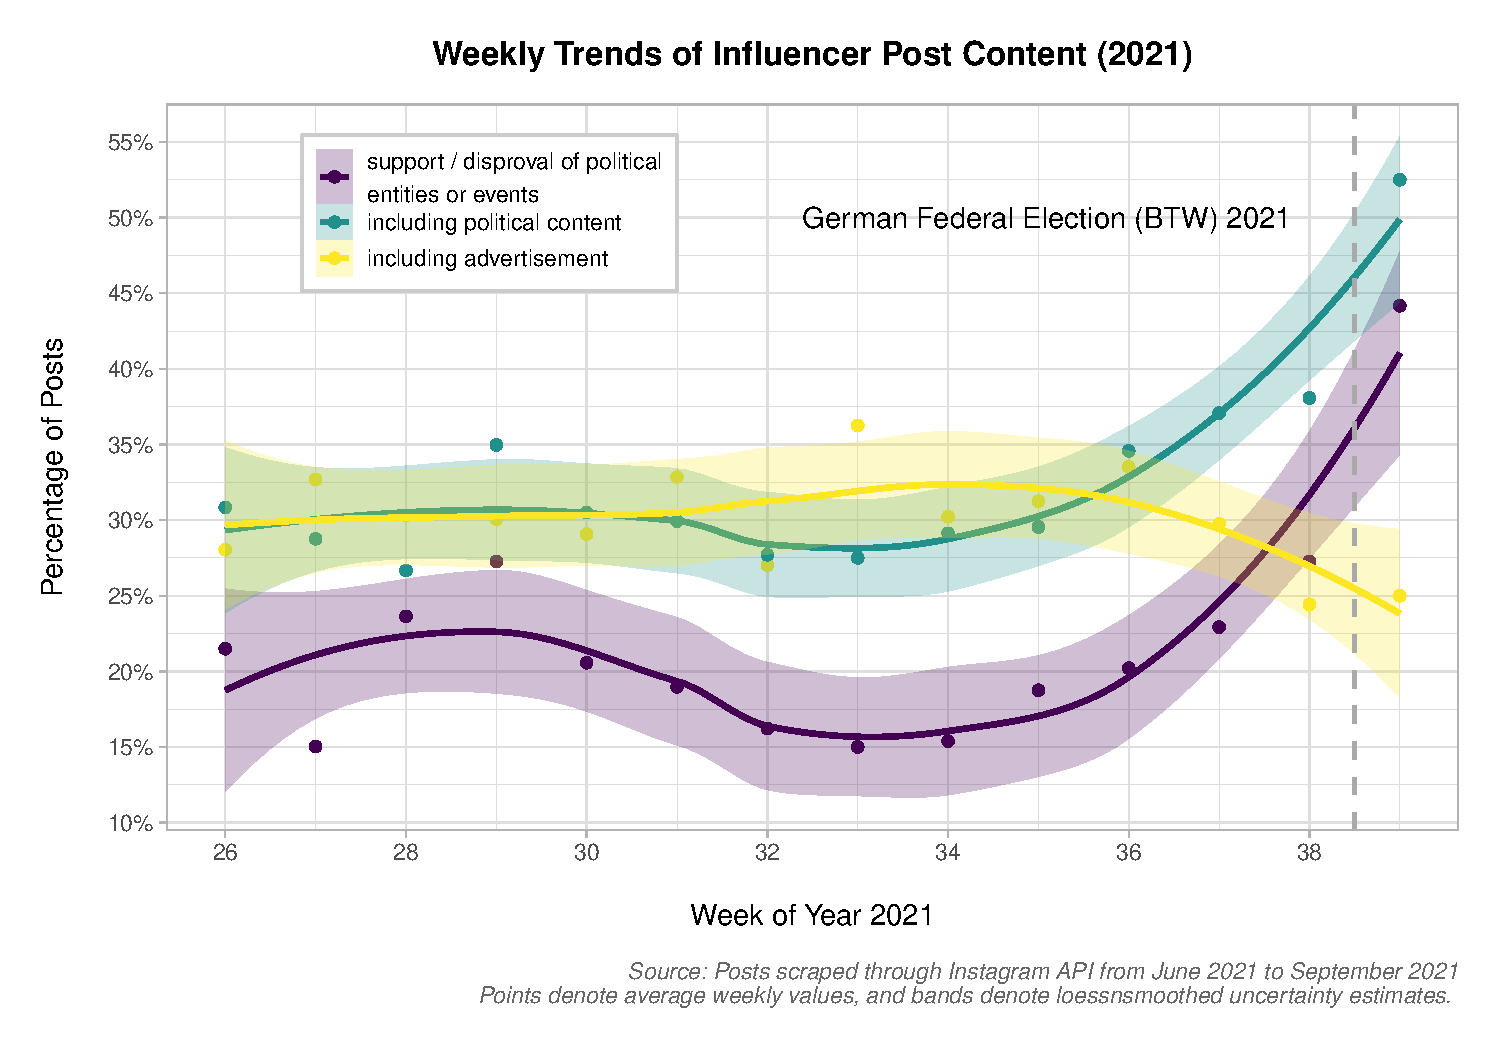
\includegraphics[width=0.85\textwidth]{fig3_rep.pdf}
		\caption{Weekly temporal trends of different post categories.}
		\label{fig:3}
	\end{figure}
	
	Figure \ref{fig:3} employs a LOESS smoothed line plot to track the weekly temporal trends of different post categories, with the vertical dashed line marking the week of the 2021 German Federal Election and the shaded bands around the lines represent the 95\% confidence intervals (uncertainty estimates). The trajectories reveal a pronounced surge in general political content as the election approaches, while explicit political endorsements remain consistently low. 
	
	The authors concluded that political influencers strategically pivot their content during campaign periods, actively broadcasting general political information while maintaining their commercial advertising baseline.
	
	\subsection{Logistic Regression Analysis}

	\lstinputlisting[language=R, firstline=147, lastline=189]{replication.R}
	
	\begin{table}[H] \centering 
		\caption{Logit Regression on Influencer Awareness and Following} 
		\label{tab:logit_models} 
		\begin{tabular}{@{\extracolsep{5pt}}lcc} 
			\\[-1.8ex]\hline 
			\hline \\[-1.8ex] 
			& \multicolumn{2}{c}{\textit{Dependent variable:}} \\ 
			\cline{2-3} 
			& Awareness of Influencers (OR) & Following Influencers (OR) \\ 
			\\[-1.8ex] & (1) & (2)\\ 
			\hline \\[-1.8ex] 
			Age & 0.985$^{***}$ & 0.952$^{***}$ \\ 
			& (0.006) & (0.007) \\ 
			& & \\ 
			Education: mid & 1.363$^{***}$ & 0.974$^{***}$ \\ 
			& (0.204) & (0.278) \\ 
			& & \\ 
			Education: high & 1.781$^{***}$ & 1.127$^{***}$ \\ 
			& (0.225) & (0.277) \\ 
			& & \\ 
			Sex: Female & 1.702$^{***}$ & 1.283$^{***}$ \\ 
			& (0.178) & (0.214) \\ 
			& & \\ 
			Number of SM used & 1.110$^{***}$ & 1.293$^{***}$ \\ 
			& (0.061) & (0.065) \\ 
			& & \\ 
			Using SM: Public figures & 1.029$^{***}$ & 1.498$^{***}$ \\ 
			& (0.095) & (0.103) \\ 
			& & \\ 
			Using SM: Brands & 0.876$^{***}$ & 1.106$^{***}$ \\ 
			& (0.095) & (0.104) \\ 
			& & \\ 
			Using SM: Entertainment & 1.296$^{***}$ & 1.342$^{***}$ \\ 
			& (0.072) & (0.105) \\ 
			& & \\ 
			Interest in politics & 1.626$^{***}$ & 0.965$^{***}$ \\ 
			& (0.083) & (0.114) \\ 
			& & \\ 
			Constant & 0.311 & 0.129 \\ 
			& (0.551) & (0.691) \\ 
			& & \\ 
			\hline \\[-1.8ex] 
			Observations & 925 & 708 \\ 
			Log Likelihood & $-$436.922 & $-$303.970 \\ 
			Akaike Inf. Crit. & 893.843 & 627.940 \\ 
			\hline 
			\hline \\[-1.8ex] 
			\textit{Note:}  & \multicolumn{2}{r}{$^{*}$p$<$0.1; $^{**}$p$<$0.05; $^{***}$p$<$0.01} \\ 
		\end{tabular} 
	\end{table} 
	
	\begin{figure}[H]
		\centering
		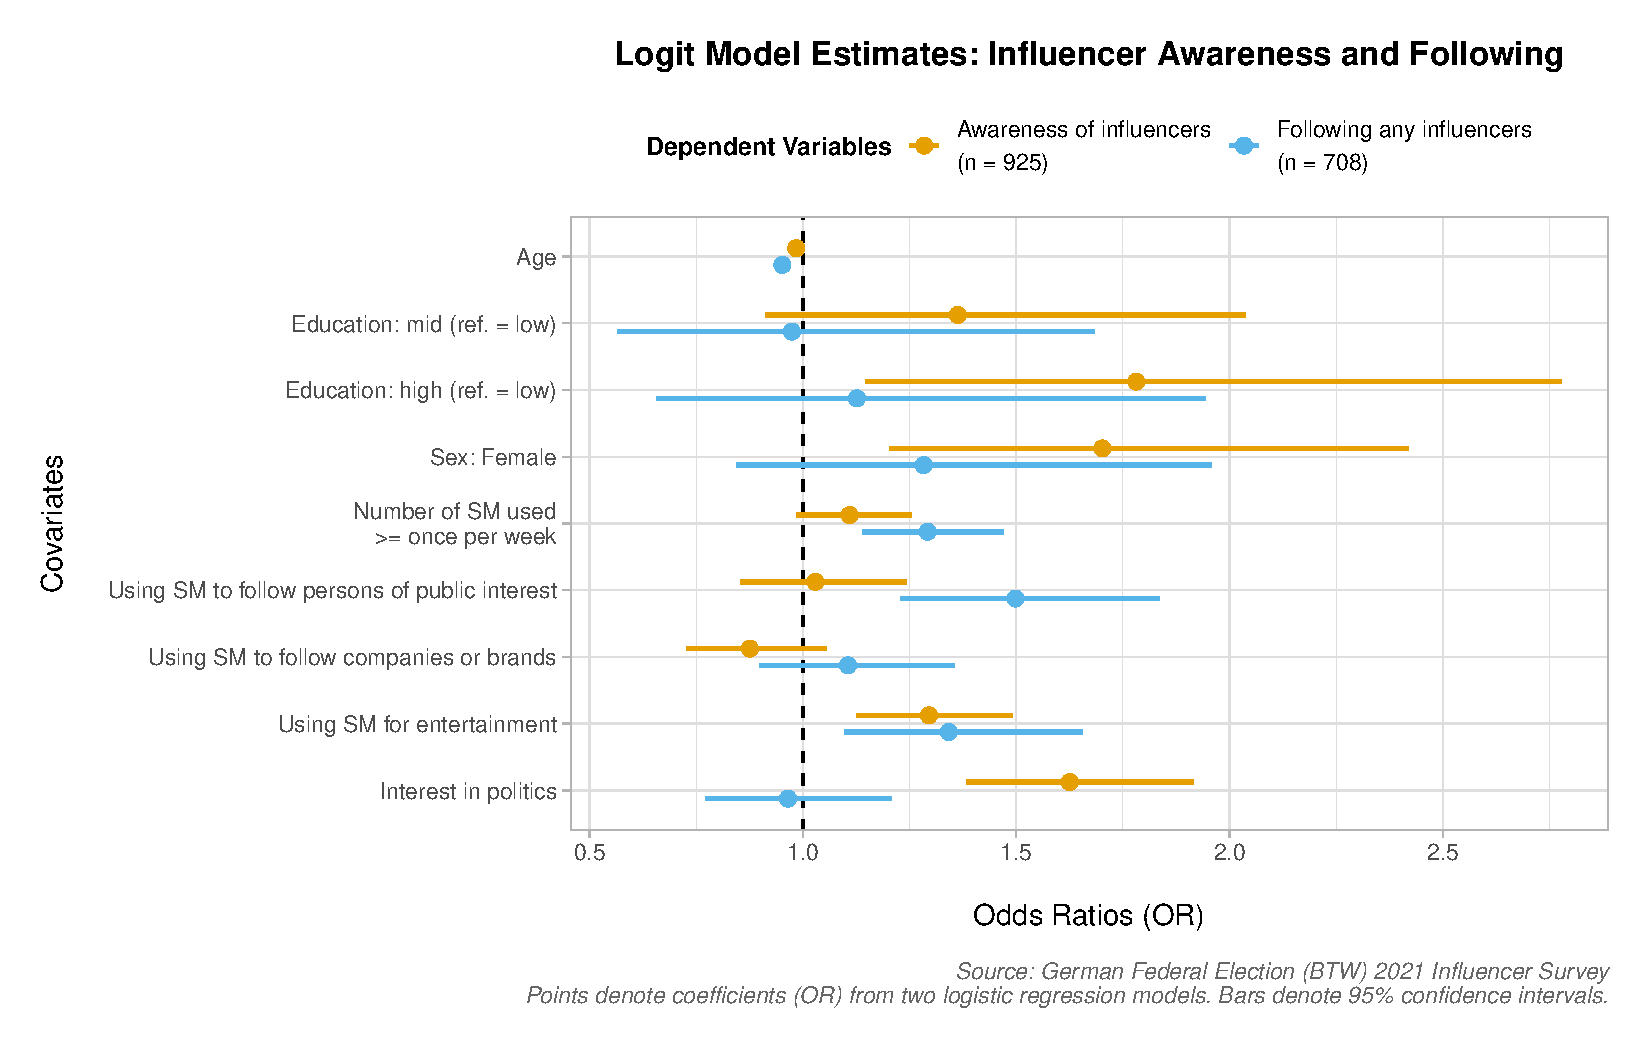
\includegraphics[width=0.85\textwidth]{fig4_rep.pdf}
		\caption{Visualizing effects of logistic models.}
		\label{fig:4}
	\end{figure}
	
	The authors aim to demonstrate that political influencers successfully reach beyond audiences who are already highly interested in politics. They argue that while political interest sparks initial awareness, non-political motivations ultimately drive the actual following behavior.
	
	Specifically, holding all other variables constant, a one-unit increase in political interest multiplies the expected odds of being aware of a political influencer by a factor of 1.63 ($p < 0.001$)on average. 
	
	Conversely, non-political drivers are significantly associated with deeper engagement:on average, holding all other covariates constant, a one-unit increase in entertainment motivation multiplies the expected odds of following a political influencer by a factor of 1.34 ($p < 0.01$).
	
	\section{Model Extension}
	
	\subsection{Model Limitations}
	While the original logistic regression provides baseline insights, it exhibits several methodological limitations:
	\begin{itemize}
		\item \textbf{Lack of Goodness-of-Fit Testing:} The original analysis omitted formal model evaluations, such as the Likelihood Ratio Test (LRT). Without comparing the full models against intercept-only null models, it is difficult to statistically verify the overall significance of the chosen predictors.
		\item \textbf{Violation of Linearity Assumptions:} Variables such as political interest (\texttt{polint}) and social media motivations (\texttt{sm04, sm05, sm07}) were treated as continuous predictors. However, as shown in the distribution plots, these 5-point Likert scale items exhibit non-uniform distributions. Simply adding them as continuous variables assumes a linear effect that may not exist in reality.
		\item \textbf{Fragmented Analysis of Dependent Variables:} The use of two separate regressions for awareness and following behavior lacks theoretical and statistical integration. Because these outcomes are highly correlated and represent different stages of the same engagement process, analyzing them in isolation obscures the transition from mere awareness to active following.
	\end{itemize}
	
	\subsection{Adding Likelihood Ratio Test}
	To evaluate the overall significance of the original regression framework, I performed a Likelihood Ratio Test (LRT) by comparing the full models against intercept-only null models. The hypotheses are defined as follows:
	
	\textbf{Model 1 (Awareness):}
	\begin{itemize}[itemsep=0em]
		\item $H_0: \beta_1 = \beta_2 = \dots = \beta_9 = 0$
		\item $H_a:$ At least one coefficient $\beta_i \neq 0$
	\end{itemize}
	
	\textbf{Model 2 (Following):}
	\begin{itemize}[itemsep=0em]
		\item $H_0: \gamma_1 = \gamma_2 = \dots = \gamma_9 = 0$
		\item $H_a:$ At least one coefficient $\gamma_i \neq 0$
	\end{itemize}
	
	{\footnotesize
		\begin{verbatim}
			Model 1null: aw_dum ~ 1
			Model 1: aw_dum ~ age + edu_cat + fem_dum + sm_cnt + sm04_num + sm05_num + sm07_num + polint
			Resid. Df Resid. Dev Df Deviance  Pr(>Chi)    
			1       924     978.56                          
			2       915     873.84  9   104.72 < 2.2e-16 ***
			---
			Model 2null: fw_dum ~ 1
			Model 2: fw_dum ~ age + edu_cat + fem_dum + sm_cnt + sm04_num + sm05_num + sm07_num + polint
			Resid. Df Resid. Dev Df Deviance  Pr(>Chi)    
			1       707     867.68                          
			2       698     607.94  9   259.74 < 2.2e-16 ***
	\end{verbatim}}
    The LRT results provide sufficient evidence to reject the null hypothesis ($H_0$) for both models ($p < 0.001$). For Model 1, the inclusion of predictors significantly reduced deviance by 104.72, while for Model 2, the deviance reduction was 259.74. This confirms that in both cases, at least one independent variable has a non-zero effect, indicating that the models with predictors possess significantly greater explanatory power than random intercept-only models.
	
	\subsection{Model Extension: Multinomial Logistic Regression}
	To address the aforementioned limitations, I re-operationalized the variables based on the conceptualization of influencer engagement proposed by Levesque et al. (2021). According to this framework, engagement is a multidimensional construct comprising \textbf{cognitive, affective/emotional, and behavioral (or activation)} dimensions. Specifically, the behavioral dimension is viewed as a spectrum of actions that include browsing (awareness), following, interacting, and sharing.
	
	Guided by this theory, I integrated awareness and following behaviors into a single categorical variable, \textit{Political Influencer Engagement}, which represents increasing levels of \textbf{behavioral activation}:
	\begin{itemize}
		\item \textbf{Level 0 (None):} No behavioral activation; unaware of influencers ($awareness=0$).
		\item \textbf{Level 1 (Aware):} Initial behavioral activation; aware of influencers but has not yet committed to following ($awareness=1, following=0$).
		\item \textbf{Level 2 (Engaged):} Advanced behavioral activation; both aware and actively following influencers ($awareness=1, following=1$).
	\end{itemize}
	
	Regarding the independent variables, I consolidated the motivations into a single factor: \textit{Entertainment and Commercial Motivation (EntMot)}. This index represents non-political drivers and was categorized into Low ($<3$), Moderate ($3-4$), and High ($\geq4$) levels to capture potential non-linear effects.\\
	
	\lstinputlisting[language=R, firstline=339, lastline=369]{replication.R}
	
	Although the dependent variable is theoretically ordered, a \textbf{Brant test} revealed a significant violation of the parallel regression assumption ($\chi^2 = 128.78, p < .001$), indicating that the relationship between each pair of outcome groups is not equal.
	
	\lstinputlisting[language=R, firstline=379, lastline=381]{replication.R}
	
	{\footnotesize
		\begin{verbatim}
			H0:The parallel regression assumption holds, where the slope coefficients are constant 
			across all binary splits of the ordinal outcome.
			Ha:The parallel regression assumption is violated.
			
			X2  df probability
			Omnibus                128.77793701  9 2.114943e-23
			age                     22.15547756  1 2.514375e-06
			edu_cat2                 0.95164361  1 3.293013e-01
			edu_cat3                 2.41168654  1 1.204326e-01
			fem_dum                  0.01774443  1 8.940287e-01
			sm_cnt                   1.93419261  1 1.643005e-01
			polint_catModerate      13.10420065  1 2.946344e-04
			polint_catHigh           9.78717495  1 1.757332e-03
			ent_mot_factorModerate  13.87985711  1 1.948759e-04
			ent_mot_factorHigh      29.36486647  1 5.995480e-08
	\end{verbatim}}
	
	Consequently, I employed an \textbf{Unordered Multinomial Logistic Regression} (Model 3) using Level 0 (None) as the baseline:
	
	\begin{equation}
		\ln\left(\frac{P(\text{Aware})}{P(\text{None})}\right) = \delta_0 + \delta_1 \text{Age} + \delta_2 \text{Edu} + \dots + \delta_6 \text{EntMot}
	\end{equation}
	
	\begin{equation}
		\ln\left(\frac{P(\text{Engaged})}{P(\text{None})}\right) = \theta_0 + \theta_1 \text{Age} + \theta_2 \text{Edu} + \dots + \theta_6 \text{EntMot}
	\end{equation}
	
	\lstinputlisting[language=R, firstline=395, lastline=404]{replication.R}
	
	\subsection{Model Results and Fit Evaluation}
	\textbf{Coefficient Interpretation:}
	
	\begin{table}[H] \centering 
		\caption{Multinomial Logistic Regression Predicting Influencer Engagement(OR)} 
		\label{tab:multi_model} 
		\begin{adjustbox}{max width=\textwidth}
			\begin{tabular}{@{\extracolsep{5pt}}lcc} 
				\toprule
				& \multicolumn{2}{c}{\textit{Dependent variable:}} \\ 
				\cmidrule{2-3} 
				& Aware (vs. None) & Engaged (vs. None) \\ 
				\midrule
				Age & 1.002 & 0.956$^{***}$ \\ 
				Education: mid & 1.404 & 1.295 \\ 
				Education: high & 1.971$^{***}$ & 2.109$^{**}$ \\ 
				Sex: Female & 1.503$^{**}$ & 2.102$^{***}$ \\ 
				Number of SM used & 1.091 & 1.384$^{***}$ \\ 
				Pol. Interest: Moderate (ref: Low) & 3.319$^{***}$ & 1.888$^{*}$ \\ 
				Pol. Interest: High (ref: Low) & 3.814$^{***}$ & 2.849$^{***}$ \\ 
				Ent. Motivation: Moderate (ref: Low) & 0.790 & 2.124$^{***}$ \\ 
				Ent. Motivation: High (ref: Low) & 0.523$^{**}$ & 2.840$^{***}$ \\ 
				Constant & 0.388$^{*}$ & 0.349$^{*}$ \\ 
				\midrule
				Akaike Inf. Crit. & 1,578.644 & 1,578.644 \\ 
				\bottomrule
				\textit{Note:} & \multicolumn{2}{r}{$^{*}$p$<$0.1; $^{**}$p$<$0.05; $^{***}$p$<$0.01} \\ 
				& \multicolumn{2}{r}{Note: The comparison category is 'None'. Coefficients represent relative Odds Ratios.} \\ 
			\end{tabular}
		\end{adjustbox}
	\end{table} 
	
	The odds ratios (OR) presented in outcome table describe the relative likelihood of moving from no awareness (None) to active engagement (Engaged).
	
	First, political interest is strongly and positively associated with influencer engagement. On average, holding all other predictors constant, the odds of being ``Engaged'' versus ``None'' for individuals with high political interest are \textbf{2.849 times} the odds of those with low interest ($p < 0.01$). 
	
	But what interesting is that entertainment and commercial motivation exhibits a similar positive trajectory. Holding other factors constant, the odds of being ``Engaged'' multiply by a factor of \textbf{2.124} for moderate motivation and \textbf{2.840} for high motivation ($p < 0.01$).
	
	This aligns with the practical context of non-elite political influencers, who strategically balance non-political and political content. Such a strategy allows them to reach a broader audience, specifically those who do not use social media primarily for the purpose of political participation.
	
	\subsection{Predicted Probabilities and Profile Analysis}
	
	To further clarify the real-world implications of the coefficients, I calculated predicted probabilities for four hypothetical audience profiles by varying political interest and entertainment motivation while holding all other covariates constant.
	
	\begin{itemize}
		\item \textbf{The Role of Political Interest:} Among individuals with high entertainment motivation, a shift from low to high political interest increases the predicted probability of awareness by $16.3\%$ (from $26.2\%$ to $42.5\%$) and engagement by $7.0\%$ (from $33.2\%$ to $40.2\%$). This confirms that pre-existing political interest remains a key driver for users to actively follow political influencers.
		
		\item \textbf{The Reach of Entertainment Motivation:} Among those with low political interest, shifting from low to high entertainment motivation results in a $22.7\%$ decrease in predicted awareness (from $48.9\%$ to $26.2\%$) but a significant $21.8\%$ increase in active engagement (from $11.4\%$ to $33.2\%$). This indicates that political influencers can effectively reach the general public by balancing political messaging with non-political personal content, successfully capturing users who do not primarily use social media for political purposes.
	\end{itemize}
	
	\begin{table}[H]
		\centering
		\caption{Predicted Probabilities of Engagement by Audience Profile (\%)}
		\label{tab:predicted_probs}
		\begin{tabular}{lccc}
			\toprule
			\textbf{Audience Profile} & \textbf{None} & \textbf{Aware} & \textbf{Engaged} \\
			\midrule
			Low Pol. Interest, Low Ent. Mot.  & 39.73 & 48.85 & 11.42 \\
			Low Pol. Interest, High Ent. Mot. & 40.66 & 26.16 & \textbf{33.18} \\
			High Pol. Interest, Low Ent. Mot. & 15.36 & 72.06 & 12.58 \\
			High Pol. Interest, High Ent. Mot. & 17.31 & 42.46 & \textbf{40.24} \\
			\bottomrule
		\end{tabular}
	\end{table}
	
	\begin{figure}[H]
		\centering
		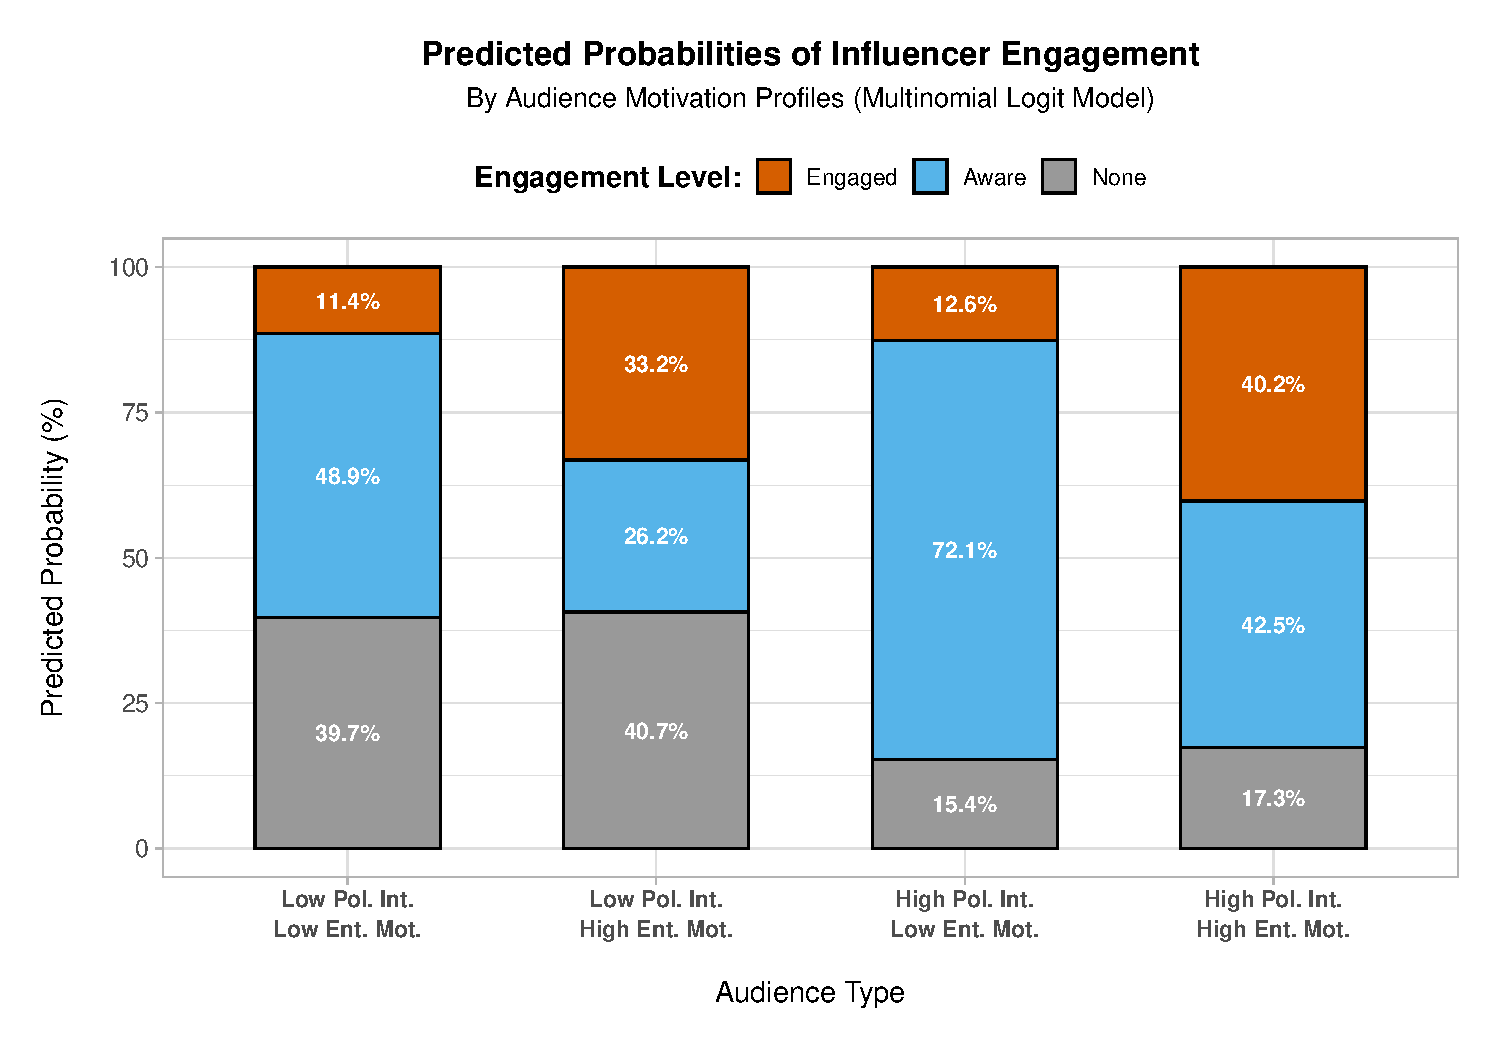
\includegraphics[width=0.85\textwidth]{fig5_predicted_probs.pdf}
	\end{figure}
	
	\lstinputlisting[language=R, firstline=437, lastline=458]{replication.R}
	
	\textbf{Fit Evaluation:} \\
	
	The model's predictive accuracy was evaluated using a confusion matrix. The overall accuracy rate was calculated 62.51\%, outperforming the null model baseline. This indicates that the model possesses certain explanatory power and provides a robust fit for predicting different levels of political influencer engagement.
	
	\begin{table}[H]
		\centering
		\caption{Confusion Matrix: Model Prediction Accuracy}
		\label{tab:confusion_matrix}
		\begin{tabular}{lcccc}
			\toprule
			& \multicolumn{3}{c}{\textbf{Predicted}} & \\
			\cmidrule(lr){2-4}
			\textbf{Actual} & \textbf{None} & \textbf{Aware} & \textbf{Engaged} & \textbf{Sum} \\
			\midrule
			\textbf{None}    & \textbf{44}  & 137 & 29  & 210 \\
			\textbf{Aware}   & 34  & \textbf{417} & 46  & 497 \\
			\textbf{Engaged} & 12  & 88  & \textbf{116} & 216 \\
			\midrule
			\textbf{Sum}     & 90  & 642 & 191 & 923 \\
			\bottomrule
		\end{tabular}
	\end{table}
		\lstinputlisting[language=R, firstline=429, lastline=435]{replication.R}
\end{document}